\begin{enumerate}

\item Use the binomial theorem (with $x=1000$ and $y=1$) to calculate
$1001^6$.

\item Find $(2x+3)^5$.

\item Find $(x^2+y^2)^6$.

\item The following diagram contains a 3-dimensional analog of
Pascal's triangle that we might call ``Pascal's tetrahedron.'' 
What would the next layer look like?

\begin{center}
\begin{picture}(0,0)%
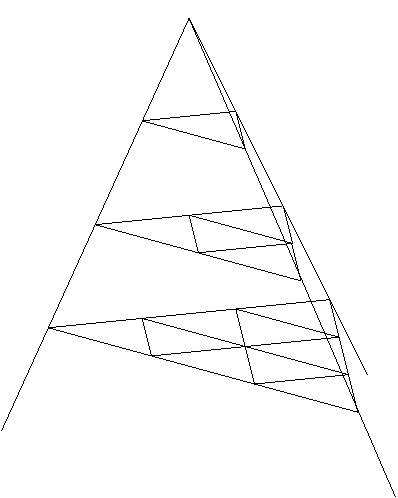
\includegraphics{figures/Pascals_tetrahedron.pdf}%
\end{picture}%
\setlength{\unitlength}{3947sp}%
%
\begingroup\makeatletter\ifx\SetFigFont\undefined%
\gdef\SetFigFont#1#2#3#4#5{%
  \reset@font\fontsize{#1}{#2pt}%
  \fontfamily{#3}\fontseries{#4}\fontshape{#5}%
  \selectfont}%
\fi\endgroup%
\begin{picture}(3174,3971)(3889,-4123)
\put(4876,-1111){\makebox(0,0)[lb]{\smash{{\SetFigFont{12}{14.4}{\familydefault}{\mddefault}{\updefault}{\color[rgb]{0,0,0}$1$}%
}}}}
\put(5851,-1036){\makebox(0,0)[lb]{\smash{{\SetFigFont{12}{14.4}{\familydefault}{\mddefault}{\updefault}{\color[rgb]{0,0,0}$1$}%
}}}}
\put(5926,-1411){\makebox(0,0)[lb]{\smash{{\SetFigFont{12}{14.4}{\familydefault}{\mddefault}{\updefault}{\color[rgb]{0,0,0}$1$}%
}}}}
\put(6526,-2536){\makebox(0,0)[lb]{\smash{{\SetFigFont{12}{14.4}{\familydefault}{\mddefault}{\updefault}{\color[rgb]{0,0,0}$1$}%
}}}}
\put(6226,-1786){\makebox(0,0)[lb]{\smash{{\SetFigFont{12}{14.4}{\familydefault}{\mddefault}{\updefault}{\color[rgb]{0,0,0}$1$}%
}}}}
\put(4501,-1936){\makebox(0,0)[lb]{\smash{{\SetFigFont{12}{14.4}{\familydefault}{\mddefault}{\updefault}{\color[rgb]{0,0,0}$1$}%
}}}}
\put(4135,-2779){\makebox(0,0)[lb]{\smash{{\SetFigFont{12}{14.4}{\familydefault}{\mddefault}{\updefault}{\color[rgb]{0,0,0}$1$}%
}}}}
\put(4955,-2642){\makebox(0,0)[lb]{\smash{{\SetFigFont{12}{14.4}{\familydefault}{\mddefault}{\updefault}{\color[rgb]{0,0,0}$3$}%
}}}}
\put(5719,-2580){\makebox(0,0)[lb]{\smash{{\SetFigFont{12}{14.4}{\familydefault}{\mddefault}{\updefault}{\color[rgb]{0,0,0}$3$}%
}}}}
\put(6631,-2841){\makebox(0,0)[lb]{\smash{{\SetFigFont{12}{14.4}{\familydefault}{\mddefault}{\updefault}{\color[rgb]{0,0,0}$3$}%
}}}}
\put(6720,-3140){\makebox(0,0)[lb]{\smash{{\SetFigFont{12}{14.4}{\familydefault}{\mddefault}{\updefault}{\color[rgb]{0,0,0}$3$}%
}}}}
\put(6782,-3494){\makebox(0,0)[lb]{\smash{{\SetFigFont{12}{14.4}{\familydefault}{\mddefault}{\updefault}{\color[rgb]{0,0,0}$1$}%
}}}}
\put(5861,-3409){\makebox(0,0)[lb]{\smash{{\SetFigFont{12}{14.4}{\familydefault}{\mddefault}{\updefault}{\color[rgb]{0,0,0}$3$}%
}}}}
\put(5026,-3184){\makebox(0,0)[lb]{\smash{{\SetFigFont{12}{14.4}{\familydefault}{\mddefault}{\updefault}{\color[rgb]{0,0,0}$3$}%
}}}}
\put(5866,-2894){\makebox(0,0)[lb]{\smash{{\SetFigFont{12}{14.4}{\familydefault}{\mddefault}{\updefault}{\color[rgb]{0,0,0}$6$}%
}}}}
\put(6319,-2377){\makebox(0,0)[lb]{\smash{{\SetFigFont{12}{14.4}{\familydefault}{\mddefault}{\updefault}{\color[rgb]{0,0,0}$1$}%
}}}}
\put(6271,-2102){\makebox(0,0)[lb]{\smash{{\SetFigFont{12}{14.4}{\familydefault}{\mddefault}{\updefault}{\color[rgb]{0,0,0}$2$}%
}}}}
\put(5330,-1817){\makebox(0,0)[lb]{\smash{{\SetFigFont{12}{14.4}{\familydefault}{\mddefault}{\updefault}{\color[rgb]{0,0,0}$2$}%
}}}}
\put(5406,-2329){\makebox(0,0)[lb]{\smash{{\SetFigFont{12}{14.4}{\familydefault}{\mddefault}{\updefault}{\color[rgb]{0,0,0}$2$}%
}}}}
\put(5441,-299){\makebox(0,0)[lb]{\smash{{\SetFigFont{12}{14.4}{\familydefault}{\mddefault}{\updefault}{\color[rgb]{0,0,0}$1$}%
}}}}
\end{picture}%

\end{center}

\item The student government at Lagrange High consists of 24 members chosen
from amongst the general student body of 210. Additionally, there
is a steering committee of 5 members chosen from amongst those in
student government. Use the multiplication rule to determine two different
formulas for the total number of possible governance structures.

\item Prove the identity
\[ \binom{n}{k} \cdot \binom{k}{r} \; = \; \binom{n}{r} \cdot \binom{n-r}{k-r} \]
combinatorially.

\item Prove the binomial theorem.

\[ \forall n \in \Naturals, \; \forall x,y \in \Reals, \; 
(x+y)^n \; = \; \sum_{k=0}^n \binom{n}{k} x^{n-k}y^k \]


\end{enumerate}

%% Emacs customization
%% 
%% Local Variables: ***
%% TeX-master: "GIAM-hw.tex" ***
%% comment-column:0 ***
%% comment-start: "%% "  ***
%% comment-end:"***" ***
%% End: ***

